\documentclass[conference]{IEEEtran}
\IEEEoverridecommandlockouts
% The preceding line is only needed to identify funding in the first footnote. If that is unneeded, please comment it out.
\usepackage{cite}
\usepackage{amsmath,amssymb,amsfonts}
\usepackage{algorithmic}
\usepackage{graphicx}
\usepackage{textcomp}
\usepackage{xcolor}
\def\BibTeX{{\rm B\kern-.05em{\sc i\kern-.025em b}\kern-.08em
    T\kern-.1667em\lower.7ex\hbox{E}\kern-.125emX}}
\begin{document}

\title{A Comparative Analysis of Image Enhancement Methods
}

\author{\IEEEauthorblockN{Shihao Piao}
\IEEEauthorblockA{\textit{Electrical and Computer Engineering} \\
\textit{University of Toronto}\\
Toronto, Canada \\
shihao.piao@mail.utoronto.ca
}
}

\maketitle
% abstract
\begin{abstract}
Image enhancement is a crucial step in digital image processing, which aims to improve the visual quality of an image by enhancing its features, such as brightness, contrast, and color. Various image enhancement methods are available, each with advantages and limitations. In this report, we present a comparative analysis of several image enhancement methods, including wiener filtering, contrast-limited adaptive histogram equalization (CLAHE), and multi-scale retinex with color restore (MSRCR). We evaluate the performance of these methods using standard image quality metrics such as peak signal-to-noise ratio (PSNR), Entropy, and lightness order error (LOE). Our experimental results show that each method has its strengths and weaknesses, and the choice of the method depends on the specific application and the desired outcome. Overall, this study provides a comprehensive analysis of image enhancement methods and serves as a valuable reference for researchers and practitioners in the field of digital image processing.
\end{abstract}

\begin{IEEEkeywords}
image enhancement, wiener filter, CLAHE, MSRCR
\end{IEEEkeywords}

% introduction
\section{Introduction}
Image enhancement is an essential task in digital image processing that aims to improve the visual quality of images by enhancing their features. The enhancement process can include adjusting brightness, contrast, color, and other attributes to make images more visually appealing and easier to interpret. The importance of image enhancement has increased over the years due to the widespread use of digital images in various fields, including medical imaging, satellite imaging, and surveillance systems.

Numerous image enhancement methods are available now, each with advantages and limitations. The choice of the method depends on the specific application and the desired outcome. Researchers have recently proposed various image enhancement methods based on histogram equalization (HE), retinex, and some filterings. These methods have been shown to be effective in enhancing images for different applications.

In this report, we present a comparative analysis of several image enhancement methods, including wiener filtering, contrast-limited adaptive histogram equalization (CLAHE), and multi-scale retinex with color restore (MSRCR). Our primary objective is to evaluate the performance of these methods using standard image quality metrics such as peak signal-to-noise ratio (PSNR), Entropy, lightness order error (LOE), and visual inspection. 

The rest of the paper is organized as follows. Section II describes the methodology used in this project, which is image enhancement methods. Section III describes the evaluation metrics. Section IV presents the experimental results and discusses the findings. Finally, Section V concludes the report.

% methods
\section{approaching methods}

%wiener filter
\subsection{Wiener Filter}
The Wiener filter is a linear signal processing method widely used in image restoration and enhancement. It is a frequency domain filter and also a linear minimum mean square error (LMMSE) filter, which means that it minimizes the difference between the output image and the ground truth image given the observed image and the noise model. The mean square error is defined below.

\begin{equation}
e^2 = E\{ (f-\hat{f})^2\}  \label{eq7}
\end{equation}

Where f is the image and $\hat{f}$ is the estimation of the image. We use a Bayesian approach based on probability and statistics to find the formula. We must find a clear target f with the highest observation probability under always observing the data g. The method of seeking the maximum posterior probability of observing the target under known data conditions is called the maximum a posteriori probability estimation method (MAP), namely:

\begin{equation}
MAP(f) = \max_f P(f\mid g) = \max_f P(g\mid f)P(f)
\label{eq8}
\end{equation}

From the mathematical point of view of MAP estimation, it is assumed that both the noise and the image obey the Gaussian distribution, and $\sigma_n^2$ and $\sigma_f^2$ represent the variance of the noise and the target, and the probability distributions are:

\begin{equation}
P(g\mid f) = \frac{1}{\sqrt{2\pi \sigma_n}} exp\{-\frac{[g(x,y)-f(x,y)*h(x,y)]^2}{2\sigma_n^2} \} \label{eq9}
\end{equation}

\begin{equation}
P(f) = \frac{1}{\sqrt{2\pi \sigma_f}} exp\{-\frac{[f(x,y)]^2}{2\sigma_f^2} \} \label{eq10}
\end{equation}

Put \eqref{eq9} and \eqref{eq10} into \eqref{eq8}, and find the extreme value, and the solution in the frequency domain is the final result.

\begin{equation}
F(u,v) = \frac{H^*(u,v)}{\lvert H^*(u,v)\rvert^2 + \frac{\sigma_n^2}{\sigma_f^2}} G(u,v) \label{eq11}
\end{equation}

The Wiener filter is especially useful for enhancing images corrupted by additive white Gaussian noise (AWGN). It works by removing noise components from an image while preserving key image features. The Wiener filter does this by taking into account the noise and the spectral properties of the image, which allows it to suppress the noise while preserving the signal.

Overall, the Wiener filter is a good choice for image enhancement and restoration in the presence of AWGN. However, its performance may be limited by the influence of the noise model and the complexity of the image structure.

%CLAHE
\subsection{CLAHE}
The CLAHE method we use is improved based on Histogram Equalization (HE). HE is a method of enhancing the contrast of an image. Its main idea is to change the histogram distribution of an image into an approximately uniform distribution, thereby enhancing the image's contrast. In HE we always use a monotonic non-linear mapping to transform image A into image B. Although histogram equalization is only an essential method in digital image processing (DIP), it is a powerful and classic algorithm. The result improved on the basis of HE is Adaptive Histogram Equalization (AHE). In the HE, the global image is directly equalized without considering the local image area. The adaptive process is to use only the histogram distribution in the local area window to construct the mapping function f during the equalization process. Since AHE is calculated by moving the window, there will be an obvious block phenomenon in the resulting image. In order to avoid the image discontinuity and over-enhancement results caused by AHE, a method of limiting the histogram distribution is introduced, that is, CLAHE. Compared with AHE, two improvements are proposed.

First, a method to constrain the histogram distribution is proposed. Consider an image's histogram, set a threshold, and clip it if a specific gray level of the histogram exceeds the threshold. Then the parts exceeding the threshold are evenly distributed to each gray level, just like Fig.~\ref{fig1}, which can make the CDF flatter. Second, an interpolation method is proposed to accelerate histogram equalization. The image is divided into blocks, and a histogram CDF is calculated for each block, which is represented in Fig.~\ref{fig2} and represents a small block with a solid black line border, referred to as a window here. Then, for each pixel of the image, find the four adjacent windows, just like the blue pixels, and calculate the mapping values of the four window histogram CDFs to the blue pixels, denoted as $f_{ul}(D),f_{ur}(D),f_{dl}(D),f_{dr}(D)$, and then proceed with bilinear interpolation obtains the final mapping value of the pixel. The formula is:

\begin{equation}
\begin{split}
f(D) = (1 - \Delta y)((1-\Delta x)f_{ul}(D) + \Delta x f_{bl}(D) )  \\
+ \Delta y ((1-\Delta x)f_{ur}(D) + \Delta x f_{br}(D))
\end{split}
\label{eq12}
\end{equation}

Where $\Delta x, \Delta y$ are the blue pixels relative to the center of the window in the upper left corner. For the red pixels in Fig.~\ref{fig2}, only the CDF of the nearest window is used for mapping; for the green pixels, the CDF mapping values of the two adjacent windows are used for interpolation. CLAHE involves the parameters of the window size, 64 tiles in 8 columns and 8 rows is a common choice\cite{4}, the size of the affected area, and the histogram threshold. The results of contrast enhancement can be better controlled by adjusting the parameters.

\begin{figure}[htbp]
\centerline{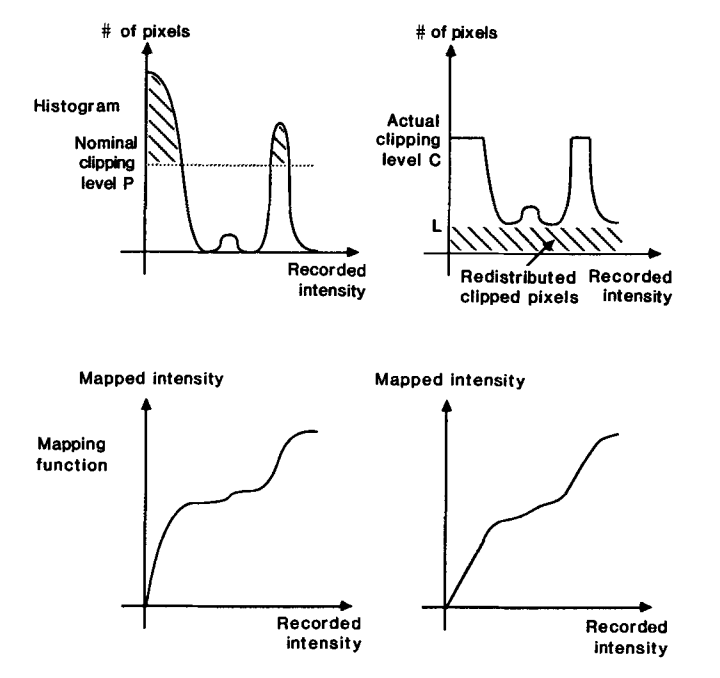
\includegraphics[width = 0.45\textwidth, height = 0.35\textwidth]{figure/CLAHE1.jpg}}
\caption{Clip Histogram\cite{3}.}
\label{fig1}
\end{figure}

\begin{figure}[htbp]
\centerline{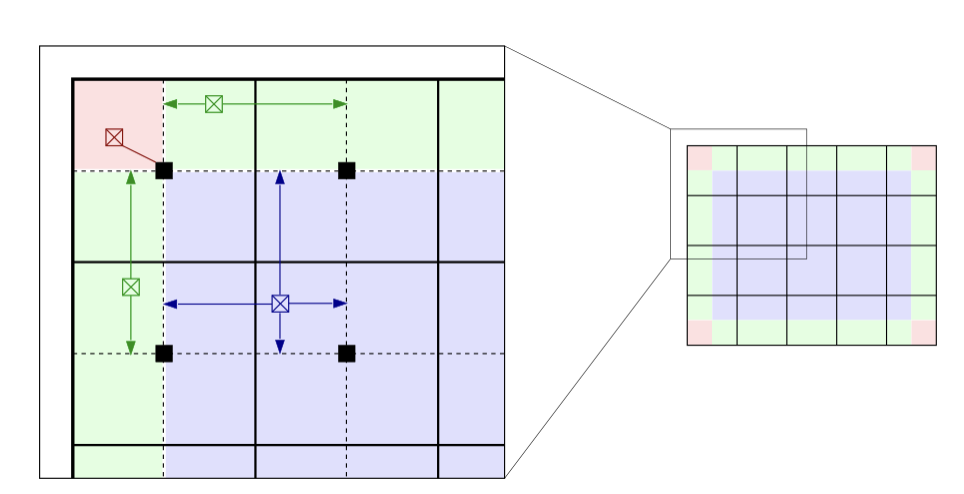
\includegraphics[width = 0.45\textwidth]{figure/CLAHE2.jpg}}
\caption{CLAHE interpolation.}
\label{fig2}
\end{figure}

%MSRCR
\subsection{MSRCR}
The MSRCR approach is based on the Retinex method. The basic content of the Retinex theory is that the color of an object is determined by the object's ability to reflect long-wave, medium-wave, and short-wave light, rather than by the absolute value of the reflected light intensity. The ability is not affected by the unevenness of illumination and has consistency; the Retinex theory is based on the consistency of color perception. An observed image I of the object the observer sees is obtained by reflecting the incident light S on the object's surface. The reflectivity R is determined by the reflected object itself and is unaffected by the incident light S. For the observed image I, the formula is expressed as:

\begin{equation}
I(x,y) = R(x,y)S(x,y) \label{eq13}
\end{equation}

The reflection component can be obtained only by estimating the brightness component S, so the estimation of S directly determines the image restoration effect. Jobson et al.\cite{5} demonstrated that the Gaussian convolution function could better estimate the brightness component from the known image I, namely

\begin{equation}
G(x,y) = k \cdot exp(-\frac{x^2+y^2}{2\sigma^2}) \label{eq14}
\end{equation}

\begin{equation}
S(x,y) = I(x,y) * G(x,y) \label{eq15}
\end{equation}

By synthesizing the above equations, we can get the expression of R in a single channel. When the value of $\sigma$ is large, the color distortion is small, but the detail recovery is poor. When the value is small, the detail recovery is good, but the color distortion is large. In order to make up for this deficiency, each channel is filtered at different scales and then summed by weight; this is called Multiscale Retinex (MSR), and the final expression is:

\begin{equation}
R_{MSR_i} = \sum_{n=1}^N w_n [\log I_i(x,y) - \log (G_n(x,y)*I_i(x,y))]\label{eq16}
\end{equation}

Because of the weighted summation, the processing time will also be longer, and different scales will be used, resulting in the restored RGB ratio being different from the original image ratio, and the color being distorted. So we introduce component ratio adjustment factors to reduce the influence of color distortion, and this is the MSRCR algorithm. The first move is to compute the chromaticity coordinates for the ith color band like \eqref{eq17}, where C is the number of spectral channels.

\begin{equation}
I_i'(x,y) = \frac{I_i(x,y)}{\sum_{j=1}^C I_j(x,y)} \label{eq17}
\end{equation}

The restored color MSR is given by\cite{6}:

\begin{equation}
R_{MSRCR_i}(x,y) = \beta \log[\alpha I_i'(x,y)] \cdot R_{MSR_i}(x,y) \label{eq18}
\end{equation}

Where $\beta$ is a gain constant, and $\alpha$ controls the strength of the nonlinearity.

%metrics
\section{metrics}

%PSNR
\subsection{PSNR}
PSNR is a widely used objective image quality metric that measures the difference between the original image and the enhanced image regarding their pixel values. It is expressed in decibels (dB) and provides a quantitative measure of the distortion introduced by the image enhancement method. A higher PSNR value indicates a smaller difference between the original and enhanced images. The PSNR is defined as follows:

\begin{equation}
PSNR = 20\times\log_{10} (255 / \sqrt{MSE})   \label{eq1}
\end{equation}

Where 255 is the maximum possible pixel value, and MSE is the mean squared error between the original and enhanced images. The MSE is computed by averaging the squared differences between corresponding pixels in the two images. PSNR is a commonly used metric in image processing applications, such as compression, denoising, and image restoration.

In our project, we use PSNR as one of the evaluation metrics to compare the performance of different image enhancement methods. We compute the PSNR values for each enhanced image with respect to the original image and compare them for different methods. A higher PSNR value indicates less distortion introduced by the enhancement method. The PSNR results, along with other evaluation metrics, provide a comprehensive analysis of the performance of each image enhancement method.

%entropy
\subsection{Entropy}
Entropy is a statistical measure that quantitatively measures the amount of information contained in an image. In digital image processing, Entropy is used as an evaluation metric to assess the randomness and complexity of an image. The entropy value of an image is computed by measuring the frequency of occurrence of each pixel value and then computing the Entropy using the following formula:

\begin{equation}
Entropy = - \sum p(x) \times \log_2p(x)   \label{eq2}
\end{equation}

Where p(x) is the probability of occurrence of the pixel value x, Entropy is often used as a quality metric for image compression, where the goal is to reduce the amount of redundant information in an image while maintaining its visual quality.

In our project, we also consider Entropy as an evaluation metric for comparing the performance of different image enhancement methods. Specifically, we compute the entropy values of the enhanced images and compare them for each method. A higher entropy value indicates a more complex and less predictable image, which implies better enhancement results. However, it is essential to note that Entropy alone cannot provide a complete measure of image quality. It should be used in conjunction with other evaluation metrics, such as PSNR, to provide a comprehensive analysis of the performance of different image enhancement methods.
%LOE
\subsection{LOE}
LOE is a perception-based evaluation metric that measures the deviation of the enhanced image's lightness order from that of the original image. Lightness order refers to the relative brightness of different regions or objects in an image. LOE is used to evaluate the performance of image enhancement methods that aim to improve the contrast or brightness of an image. The calculation formula is defined as follows:

\begin{equation}
L(x,y) = \max_{c\in\{r,g,b\}} I^c(x,y)  \label{eq3}
\end{equation}

\begin{equation}
U(x,y) = \begin{cases}
1, x\geq y \\
0, else
\end{cases}  \label{eq4}
\end{equation}

\begin{equation}
RD(x,y) = \sum_{i=1}^m \sum_{j=1}^n U((L(x,y) , L(i,j)) \oplus (L_e(x,y) , L_e(i,j)))  \label{eq5}
\end{equation}

\begin{equation}
LOE = \frac{1}{m\times n}\sum_{i=1}^m \sum_{j=1}^n RD(i,j)  \label{eq6}
\end{equation}

Where L(x,y) means the max pixel value among all channels, m, and n is the height and width of the image, respectively.

In our project, we also consider LOE as an evaluation metric to complement the other objective and subjective evaluation metrics. We compute the LOE values for each enhanced image and compare them for different image enhancement methods. A lower LOE value indicates a smaller deviation in the lightness order between the original and enhanced images, which implies better image quality. The LOE results, along with other evaluation metrics, provide a comprehensive analysis of the performance of each image enhancement method. 

However, it is essential to note that LOE is only applicable to images with distinct regions or objects with different lightness values. For images with uniform lightness values, LOE may not provide a meaningful measure of image quality.
%results
\section{experimental results}

The experimental part, we divided it into two parts, one part is grayscale images, and the other part is RGB images. For the judgment of whether the result is good or bad, we will first judge based on the subjective judgment of vision and then combine the value of the metric because most images do not have a ground truth image, so the metric cannot describe the image very accurately and can only provide a reference. In the first part of grayscale images, we experimented with three kinds of images, namely the restoration of images with noise and blur effects and the enhancement of vague images and medical images.

As shown in Fig.~\ref{fig3}, for noise images, the best result of visual judgment is obtained by wiener filtering. Although CLAHE should be the best result according to the data of Table~\ref{tab1}, there is not much difference between the two values, and the image brightness after CLAHE processing is too high, so we think Wiener is the best result. As shown in Fig.~\ref{fig4}, CLAHE and MSRCR both perform well according to the results of visually enhancing vague images. According to the value of Table~\ref{tab1}, we can see that CLAHE is more different from the original image and contains more information, and the image is more complex than MSRCR, so CLAHE is the best choice. As shown in Fig.~\ref{fig5}, for the enhancement of medical images, both Wiener and CLAHE have good results according to visual inspection. According to the metric value from Table~\ref{tab1}, CLAHE contains more information, so it is considered that CLAHE is the best choice.

For the enhanced results of the low light image, it can be seen from Fig.~\ref{fig6} that the results of MSRCR are the best. Because Wiener cannot handle color images, we removed the result of Wiener and added LOE to the metric. The natural preservation ability of the image reflected by LOE, the smaller the value, the better the brightness order of the image, and the more natural it looks. The comparison in Table~\ref{tab2} shows that the LOE value of MSRCR is smaller than that of CLAHE, and the remaining PSNR and Entropy methods are not much worse, so MSRCR is the best choice for processing low-light images.

\begin{figure}[htbp]
\centerline{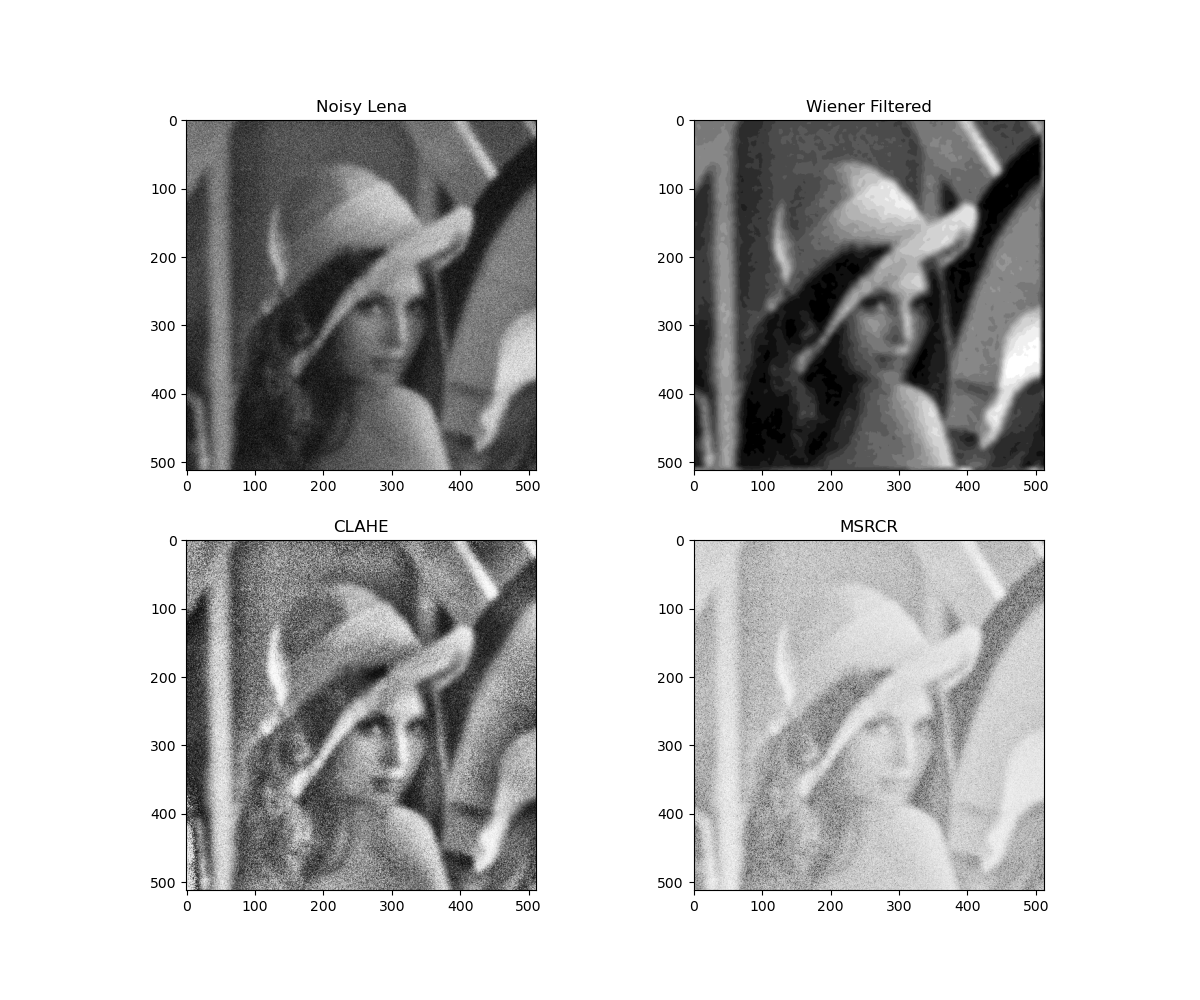
\includegraphics[width = 0.5\textwidth, height = 0.4\textwidth]{figure/lena.png}}
\caption{Noisy and blur image restoration.}
\label{fig3}
\end{figure}

\begin{figure}[htbp]
\centerline{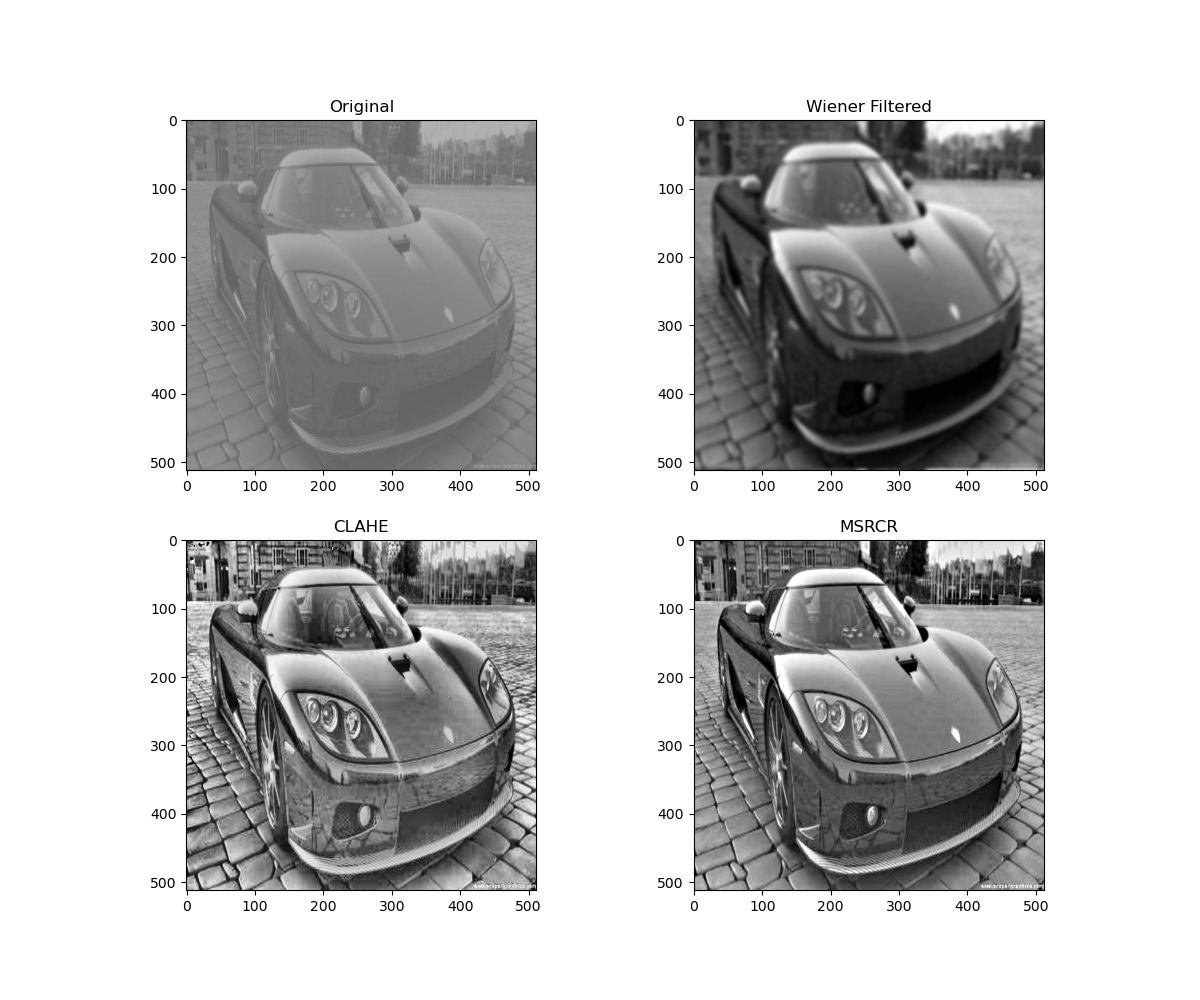
\includegraphics[width = 0.6\textwidth, height = 0.4\textwidth]{figure/car.png}}
\caption{Vague image enhancement.}
\label{fig4}
\end{figure}

\begin{figure}[htbp]
\centerline{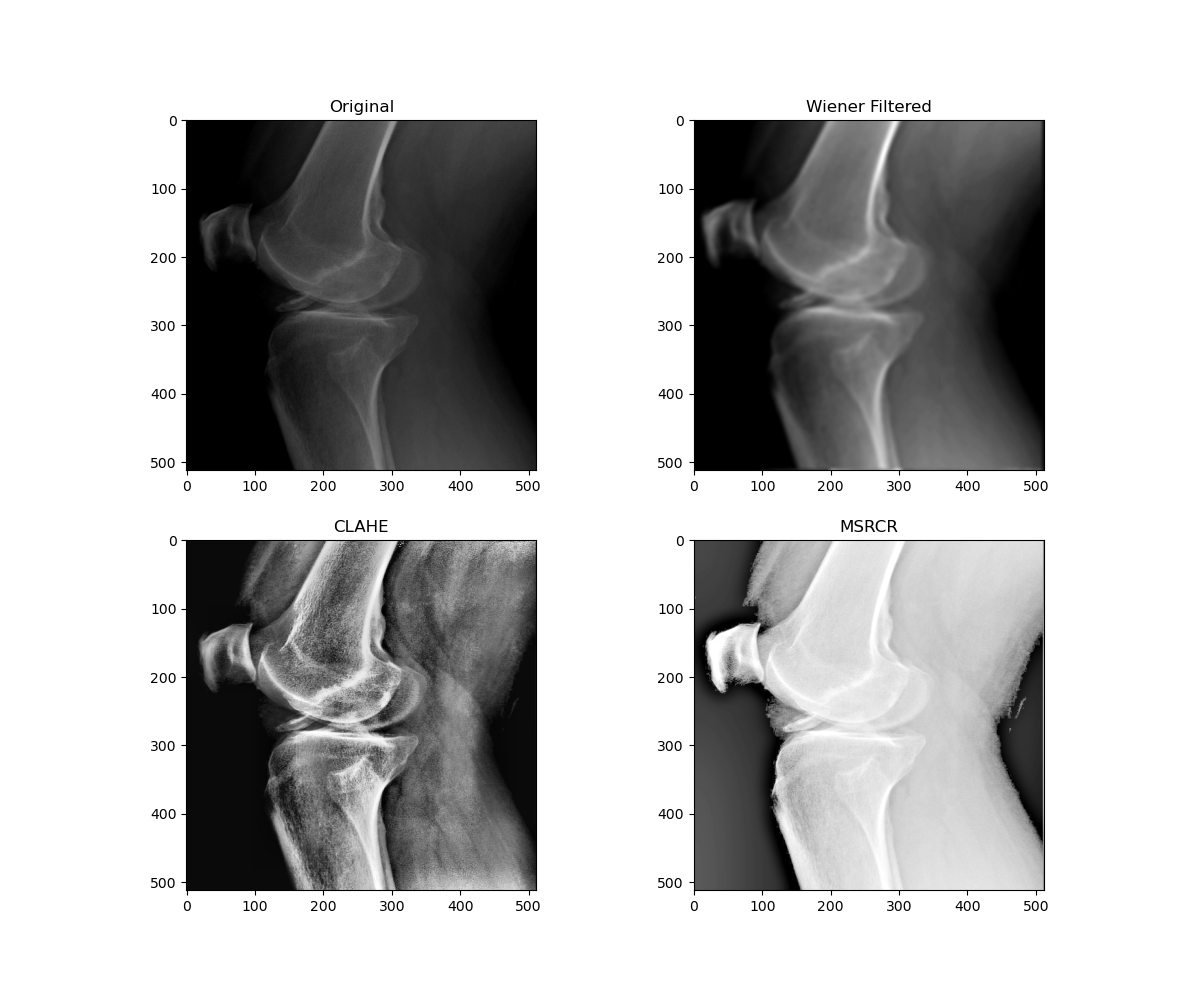
\includegraphics[width = 0.45\textwidth, height = 0.5\textwidth]{figure/medical.png}}
\caption{Medical image enhancement.}
\label{fig5}
\end{figure}

\begin{table}[htbp]
\caption{metric values for different gray images}
\begin{center}
\begin{tabular}{|c|c|c|c|}
\hline
\multicolumn{4}{|c|}{\textbf{Noisy and blur image}} \\
\hline
\textbf{Metric} & \textbf{\textit{Wiener filter}}& \textbf{\textit{CLAHE}}& \textbf{\textit{MSRCR}} \\
\hline
PSNR (dB)& 28.35& 27.84& 27.82 \\
\hline
Entropy & 7.65 & 7.81 &6.83 \\
\hline
\multicolumn{4}{|c|}{\textbf{Vague image}} \\
\hline
\textbf{Metric} & \textbf{\textit{Wiener filter}}& \textbf{\textit{CLAHE}}& \textbf{\textit{MSRCR}} \\
\hline
PSNR (dB)& 27.64& 27.89& 27.97 \\
\hline
Entropy & 7.67 & 7.81 &6.92 \\
\hline
\multicolumn{4}{|c|}{\textbf{Medical image}} \\
\hline
\textbf{Metric} & \textbf{\textit{Wiener filter}}& \textbf{\textit{CLAHE}}& \textbf{\textit{MSRCR}} \\
\hline
PSNR (dB)& 28.72& 27.87& 27.66 \\
\hline
Entropy & 6.44 & 6.93 &6.88 \\
\hline
\end{tabular}
\label{tab1}
\end{center}
\end{table}

\begin{figure}[htbp]
\centerline{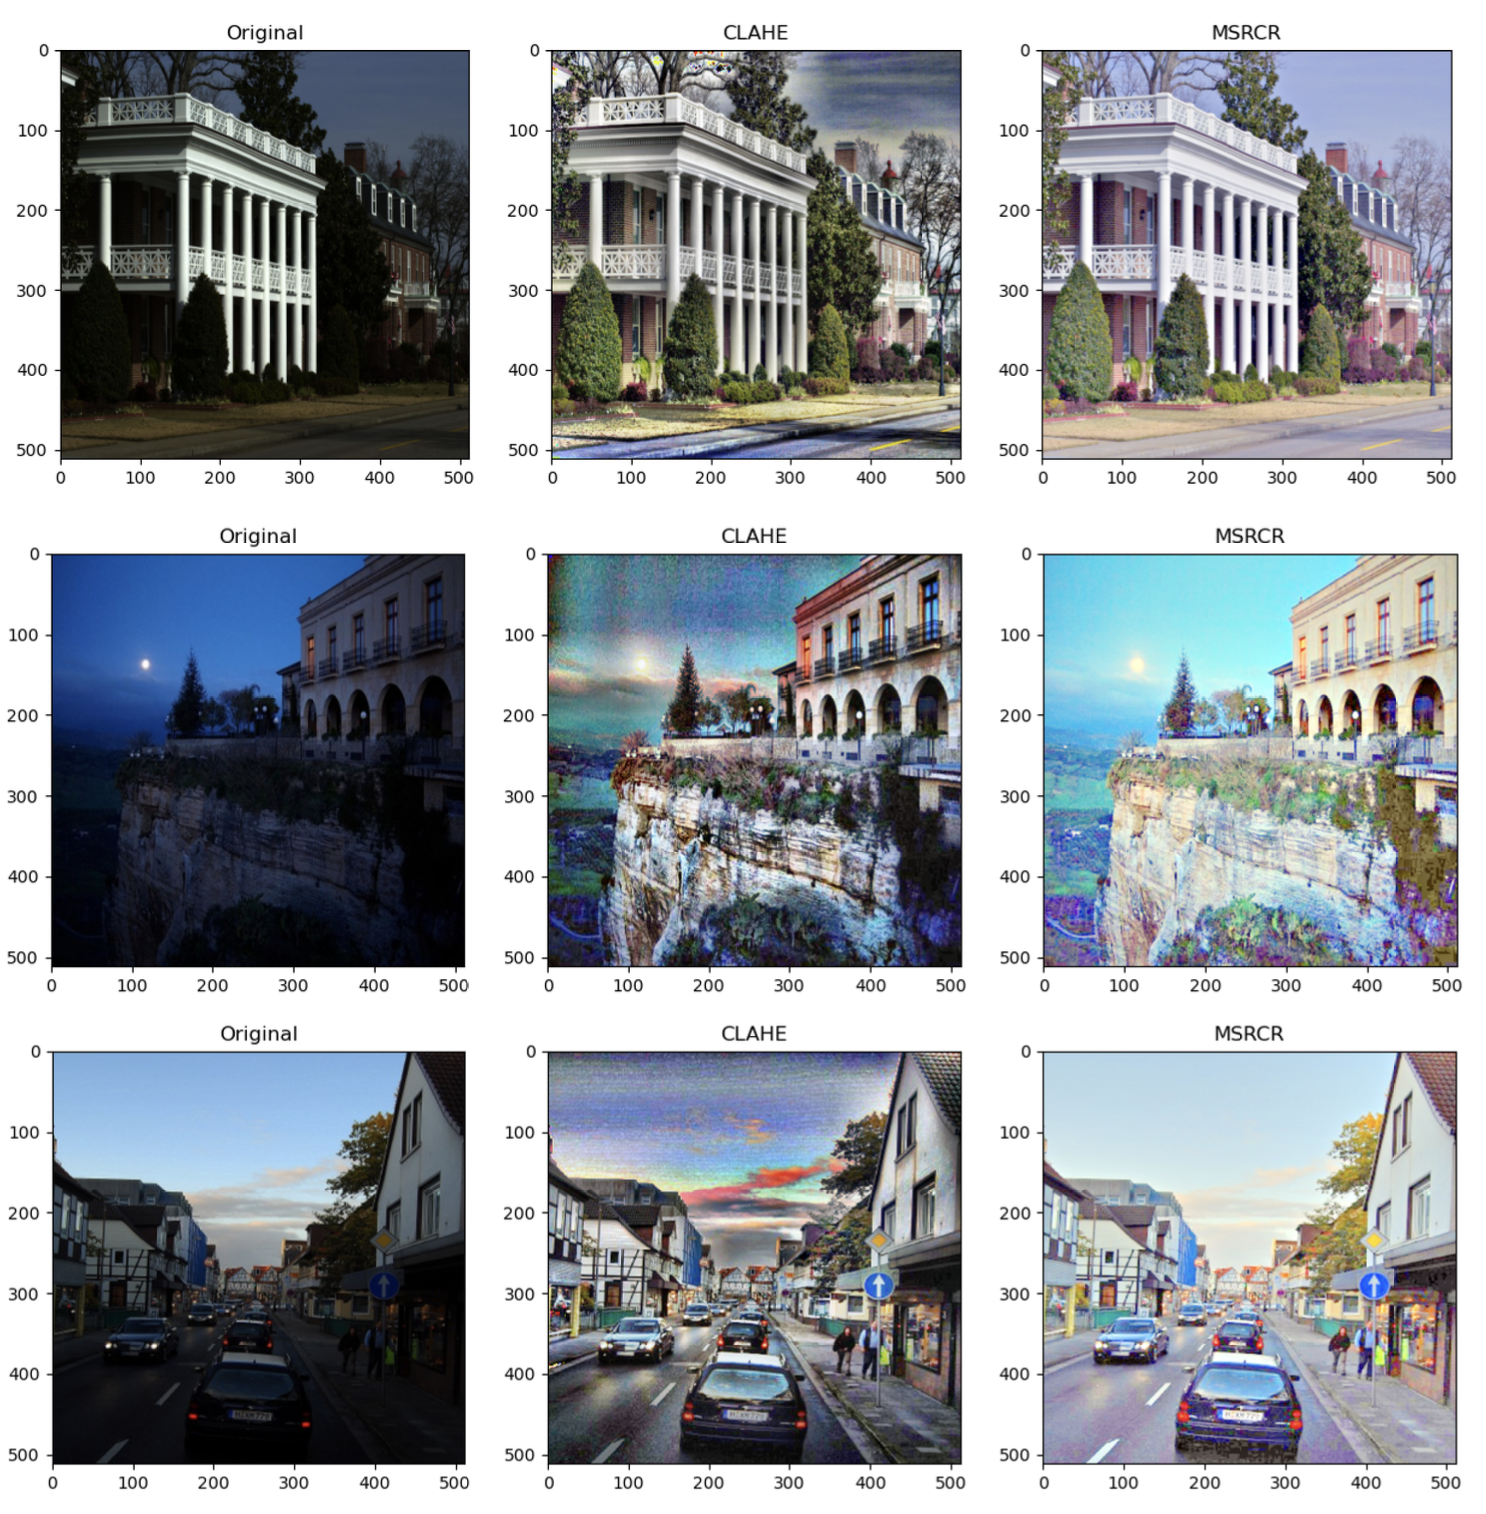
\includegraphics[width = 0.45\textwidth, height = 0.45\textwidth]{figure/collect.png}}
\caption{Low-light image enhancement.}
\label{fig6}
\end{figure}

\begin{table}[htbp]
\caption{metric values for different RGB images}
\begin{center}
\begin{tabular}{|c|c|c|}
\hline
\multicolumn{3}{|c|}{\textbf{Low light image 1}} \\
\hline
\textbf{Metric} &  \textbf{\textit{CLAHE}}&\textbf{\textit{MSRCR}} \\
\hline
PSNR (dB)& 27.95& 28.12 \\
\hline
Entropy & 7.92 & 7.69 \\
\hline
LOE & 781.52 & 425.5 \\
\hline
\multicolumn{3}{|c|}{\textbf{Low light image 2}} \\
\hline
\textbf{Metric} &  \textbf{\textit{CLAHE}}&\textbf{\textit{MSRCR}} \\
\hline
PSNR (dB)& 27.76& 27.85 \\
\hline
Entropy & 7.81 & 7.47 \\
\hline
LOE & 737.88 & 363.46 \\
\hline
\multicolumn{3}{|c|}{\textbf{Low light image 3}} \\
\hline
\textbf{Metric} &  \textbf{\textit{CLAHE}}&\textbf{\textit{MSRCR}} \\
\hline
PSNR (dB)& 27.79& 27.78 \\
\hline
Entropy & 7.84 & 7.38 \\
\hline
LOE & 493.98 & 422.04 \\
\hline
\end{tabular}
\label{tab2}
\end{center}
\end{table}


%conclusion
\section{conclusion}
In this project, we comprehensively compared three image enhancement methods, Wiener filter, CLAHE, and MSRCR. We evaluate their performance using objective metrics such as PSNR, Entropy, and LOE, as well as subjective evaluations by human visual inspection.

From our analysis, each method has advantages and limitations. The Wiener filter is a powerful image enhancement and restoration tool, especially in additive white Gaussian noise and blur cases, but it cannot handle RGB pictures. CLAHE helps enhance contrast but can lead to the over-amplification of noise. CLAHE works well for vague image and medical image enhancement. MSRCR performs well when enhancing low-light images, but when processing grayscale images; it will cause the image to be over-enhanced and look unnatural.

In general, choosing an appropriate image enhancement method depends on the specific application and the characteristics of the image and noise. This project provides a comprehensive comparison of different image enhancement methods that can help researchers and practitioners choose the most suitable method for their specific application.


\begin{thebibliography}{00}
\bibitem{1} Tran, Le-Anh. (2019). Image Processing Course Project: Image Filtering with Wiener Filter and Median Filter. 10.13140/RG.2.2.15700.65921.
\bibitem{2} Furuya H, Eda S, Shimamura T. Image restoration via Wiener filtering in the frequency domain[J]. WSEAS transactions on signal processing, 2009, 5(2): 63-73.
\bibitem{3}Pizer S M, Amburn E P, Austin J D, et al. Adaptive histogram equalization and its variations[J]. Computer vision, graphics, and image processing, 1987, 39(3): 355-368.
\bibitem{4}K. Zuiderveld: Contrast Limited Adaptive Histogram Equalization. In: P. Heckbert: Graphics Gems IV, Academic Press 1994, ISBN 0-12-336155-9
\bibitem{5}Jobson D J, Rahman Z, Woodell G A. Properties and performance of a center/surround retinex[J]. IEEE transactions on image processing, 1997, 6(3): 451-462.
\bibitem{6}Ana Belén Petro, Catalina Sbert, and Jean-Michel Morel, Multiscale Retinex, Image Processing On Line, (2014), pp. 71–88. https://doi.org/10.5201/ipol.2014.107

\end{thebibliography}



\end{document}
